\section{Introduction}

% A few sentences placing the work in high-level context. Limit it to a few paragraphs at most; your report is on reproducing a piece of work, you don’t have to motivate that work.

Recent developments of deep neural networks have resulted in black-box models whose transparency plays a key role in explaining decisions made in fields such as healthcare, finance, or justice. The demand for methods that interpret entangled models grows with their complexity, especially now when unsupervised learning takes over in the form of autoencoders (\cite{BootstrapYourOwnLatent}, \cite{anomalydetectionexample}, \cite{clusteringautoencoders}). At this moment, there are ways for explaining models in a supervised setting, such as feature and example importance analysis. Feature importance analysis can highlight the contribution a feature has towards a decision made by a model (\cite{GradientShap}, \cite{saliency}, \cite{IntegratedGradients}). Similarly, example importance analysis highlights the major data points that influence the training (\cite{dknn}, \cite{tracIn}, \cite{simplex}). These methods are researched in supervised environments, yet in an unsupervised setting, the problem remains unsolved. 
\\ \\
To address this issue, Crabb{\'e} and van der Schaar introduce "Label-Free Explainability for Unsupervised Models" \cite{originalpaper}. They extend previous explainability methods introduced in the context of supervised learning such as feature and example importance to the unsupervised and self-supervised regimes by defining a wrapper function to these methods. In addition, the authors claim that representation-based example importance introduced in supervised contexts can be easily extended to a label-free setting by replacing the supervised representation map with an unsupervised one. To show that their approach is effective and reliable the authors performed several experiments covering both unsupervised and self-supervised approaches. 
\\ \\ 
In this research, we aim to evaluate the reproducibility of the paper by replicating their experiments, and by investigating further with different settings to reinforce their claims.

\section{Scope of reproducibility}
\label{sec:claims}

% Introduce the specific setting or problem addressed in this work, and list the main claims from the original paper. Think of this as writing out the main contributions of the original paper. Each claim should be relatively concise; some papers may not clearly list their claims, and one must formulate them in terms of the presented experiments. (For those familiar, these claims are roughly the scientific hypotheses evaluated in the original work.)

% A claim should be something that can be supported or rejected by your data. An example is, ``Finetuning pretrained BERT on dataset X will have higher accuracy than an LSTM trained with GloVe embeddings.''
% This is concise, and is something that can be supported by experiments.
% An example of a claim that is too vague, which can't be supported by experiments, is ``Contextual embedding models have shown strong performance on a number of tasks. We will run experiments evaluating two types of contextual embedding models on datasets X, Y, and Z."

% This section roughly tells a reader what to expect in the rest of the report. Clearly itemize the claims you are testing:
% \begin{itemize}
%     \item Claim 1
%     \item Claim 2
%     \item Claim 3
% \end{itemize}

% Each experiment in Section~\ref{sec:results} will support (at least) one of these claims, so a reader of your report should be able to separately understand the \emph{claims} and the \emph{evidence} that supports them.

%\jdcomment{To organizers: I asked my students to connect the main claims and the experiments that supported them. For example, in this list above they could have ``Claim 1, which is supported by Experiment 1 in Figure 1.'' The benefit was that this caused the students to think about what their experiments were showing (as opposed to blindly rerunning each experiment and not considering how it fit into the overall story), but honestly it seemed hard for the students to understand what I was asking for.}


The authors developed a new framework called label-free explainability, which allows to extend linear feature importance and example importance methods to the unsupervised setting. They proved the following properties of this framework: completeness and invariance with respect to latent symmetries. Moreover, the authors experiment with pretext tasks as a use case for label-free explainability. Lastly, they evaluated qualitatively and quantitatively whether the generative factor associated with each latent unit is identifiable by using the saliency map of its latent unit with disentangled VAEs. In this study, we will verify the following claims of the original paper: 

\begin{enumerate}[label=\textbullet, ref=\arabic*]
   \item \textbf{Claim 1}: Defining an auxiliary scalar function as a wrapper around the label-free black-box permits to compute feature importance by utilizing attributions such as Gradient Shap \cite{GradientShap}, Integrated Gradients \cite{IntegratedGradients}, and Saliency \cite{saliency}. \label{claim1}
   \item \textbf{Claim 2}: Label-free extension for example importance allows to identify salient training examples that are related to test examples one wants to explain by utilizing loss and representation-based methods.\label{claim2}
    %Interpretability of saliency maps associated to individual latent units is unrelated to the strength of disentanglement between the units.
   \item \textbf{Claim 3}: Given the notion of label-free explainability, different pretext tasks do not produce interchangeable representations in self-supervised learning.\label{claim3}
   \item \textbf{Claim 4}: The ability to understand the significance of certain features in a model, represented by saliency maps, is not dependent on how well the latent units in the model are separated or disentangled from one another.\label{claim4}
\end{enumerate}

The rest of this report is organized in the following way: in section 3 we present the methodology by introducing the models, datasets, and the experimental setup used in our study, section 4 contains the results of the performed experiments, and in section 5 we discuss our experience and conclude on the results.


\section{Methodology}

% Explain your approach - did you use the author's code, or did you aim to re-implement the approach from the description in the paper? Summarize the resources (code, documentation, GPUs) that you used.
The PyTorch implementation for reproducing the experiments is provided by the authors. By using their experimental settings, we were able to reproduce all the results from the paper. To conduct further experiments for the generalizability of the paper, we extended the provided code. We ran the experiments on Nvidia TITAN RTX GPU.


\subsection{Model descriptions}
% Include a description of each model or algorithm used. Be sure to list the type of model, the number of parameters, and other relevant info (e.g. if it's pretrained). 

% It is important to describe two popular post-hoc interpretability techniques used in the paper: label-free feature importance and label-free example importance which respectively identify essential features and examples to form representations at inference time. 

% \vspace{\baselineskip}
\subsubsection{Feature Importance}

The extension to label-free feature importance methods proposed by the authors required defining an auxiliary scalar function $g_x$ as a wrapper around black box function $f$. That function is then fed to any importance method $a_i$:

\begin{equation}
    b_i\left(f,x\right)=a_i\left(g_x,x\right)
\end{equation}
\begin{center}
    $g_x:X\rightarrow\mathbb{R}\ \ \ \text{such\ that\ for\ all}\ \widetilde{x}\in X:$
\end{center}
\begin{equation}
     g_x\left(\widetilde{x}\right)=\left\langle f\left(x\right),f\left(\widetilde{x}\right)\right\rangle_H .
\end{equation}

% \vspace{\baselineskip}
Moreover, the authors proposed to weight importance scores in label-free environments by using activation scores from the previous layer. For a more detailed explanation refer to section 2.2 of the original paper \cite{originalpaper}.

% \vspace{\baselineskip}
\subsubsection{Example Importance}

In terms of the example importance, the authors split the methods into two families: loss-based and representation-based. For the former, in a supervised setting the importance score is assigned to each training example according to the influence on the loss when they are removed. In terms of the label-free setting, we want to train our model using a label-free loss $L = X \times \Theta \rightarrow H$. This is usually not enough as the authors explain, due to the fact that the importance scores that are computed can include irrelevant parts of the black-box. To solve that problem the authors split the parameter space $\Theta = \Theta_r \times \Theta_{irr}$, where \textit{r} corresponds to the relevant parameters and \textit{irr} to irrelevant parameters. This leads to the following equation: 

\begin{equation}
    c^n\left(f_{\theta_r},x\right)=\delta_{\theta_r}^nL\left(x,\theta_*\right) .
\end{equation}

% Since we want to calculate the shift of the loss after removing one example from the training dataset, we can use the following function without retraining the model \cite{koh2017}:

% \begin{equation}
% \delta_\theta^n L\left(z, \theta_*\right) \approx \frac{1}{N}\left\langle\nabla_\theta L\left(z, \theta_*\right), H_{\theta_*}^{-1} \nabla_\theta L\left(z^n, \theta_*\right)\right\rangle_{\Theta} .
% \end{equation}

Using this equation we assume that the loss depends only on a single input example which is not true for contrastive losses \cite{simclrref}. Due to the fact that there is no apparent extension of loss-based example importance for settings with contrastive losses, the authors proposed a label-free modification of the representation-based example importance method. Representation-based methods attribute to each training example a score by analyzing the example's latent representation. For experiments with the CIFAR-10 dataset, we used the SimCLR model. For the ECG5000 dataset, a Recurrent Autoencoder with an encoder, two LSTMs, and a final linear layer was used.
Moreover, for MNIST we used an autoencoder for each pretext task. Lastly, for disentangled VAEs we used $\beta$-VAE \cite{betavae} and TC-VAE \cite{tcvae}. Descriptions of the models and hyperparameters used can be found in the Appendix \ref{appendix:models}

\subsection{Datasets}

In order to check the consistency of the feature and example importance methods, the authors fitted the models described above on 3 datasets: MNIST \citep{mnist}, ECG5000 \citep{ecg} and CIFAR-10 \citep{cifar10}. They also challenged the interpretability of disentangled representations by training the β-VAE and TC-VAE on both MNIST and dSprites \citep{dsprites}. We extended the analysis by also using the Fashion MNIST dataset \citep{fashion} to perform consistency and pretext tests. An overview of the most important information on the datasets can be seen in Table \ref{table-datasets} and more details about them can be found in Appendix \ref{appendix:datasets}.


% For each dataset include 1) relevant statistics such as the number of examples and label distributions, 2) details of train / dev / test splits, 3) an explanation of any preprocessing done, and 4) a link to download the data (if available).


\begin{table}[H]
\begin{tabular}{lcccl}
\hline
Datasets and links & \multicolumn{2}{c}{Samples}                             & \multicolumn{1}{l}{Classes} & Description                         \\ \cline{2-3}
                   & Train                      & Test                       & \multicolumn{1}{l}{}        &                                     \\ \hline
\href{http://yann.lecun.com/exdb/mnist/}{MNIST}              & \multicolumn{1}{l}{60 000} & 10 000                     & 10                          & Grayscale images of 0-9 digits.     \\
\href{https://www.cs.toronto.edu/~kriz/cifar.html}{CIFAR-10}           & \multicolumn{1}{l}{50 000} & 10 000                     & 10                          & RGB images of objects.              \\
\href{https://github.com/zalandoresearch/fashion-mnist}{Fashion MNIST}      & \multicolumn{1}{l}{60 000} & \multicolumn{1}{l}{10 000} & 10                          & Grayscale images of clothing items. \\
\href{https://github.com/deepmind/dsprites-dataset}{dSprites}           & \multicolumn{2}{c}{737 280}                             & -                           & Synthetic images of 2D shapes.      \\
\href{http://www.timeseriesclassification.com/description.php?Dataset=ECG5000}{ECG5000}            & \multicolumn{2}{c}{5 000}                               & 2                           & Time series of heart rates.         \\ \hline
\end{tabular}
\caption{\label{table-datasets}Overview of the datasets used for validating the proposed methods in the label-free setting.}
\end{table}

\subsection{Hyperparameters}

% Describe how the hyperparameter values were set. If there was a hyperparameter search done, be sure to include the range of hyperparameters searched over, the method used to search (e.g. manual search, random search, Bayesian optimization, etc.), and the best hyperparameters found. Include the number of total experiments (e.g. hyperparameter trials). You can also include all results from that search (not just the best-found results).

The authors of the original paper provided hyperparameters settings for all the experiments they performed. To match the results of the experiments we have decided to follow the setup used by them. For additional experiments, we used the same setup of hyperparameters to ensure the comparability of the results. 

\subsection{Experimental setup and code}
% Mara

% Include a description of how the experiments were set up that's clear enough a reader could replicate the setup. 
% Include a description of the specific measure used to evaluate the experiments (e.g. accuracy, precision@K, BLEU score, etc.). 
% Provide a link to your code.

The code developed by Crabb{\'e} and van der Schaar is available online on \href{https://github.com/JonathanCrabbe/Label-Free-XAI}{GitHub}. It mainly reflects the setup described in Appendix B of their paper, and therefore constitutes the base we use for verifying their claims. We use the same metrics as in the original paper to compute the feature and example importance: latent shift for feature importance and similarity rate for example importance.


In addition, to support \textbf{\hyperref[claim1]{claim 1}} we experiment with a pixel-flipping approach for masking CIFAR-10 (method referenced by the authors in the paper), instead of blurring as masking. We visually analyze the results and observe the trends in the plots. For addressing \textbf{\hyperref[claim1]{claim 1}}, \textbf{\hyperref[claim3]{claim 3}} and \textbf{\hyperref[claim4]{claim 4}}  we experiment with a different predefined attribution method from PyTorch, Integrated Gradients, in the context of the pretext and VAE experiments where Gradient Shap is initially used on the MNIST dataset. We use the Pearson correlation and the plots produced to quantitatively and qualitatively analyze the results and compare them with those from the original paper. To further challenge \textbf{\hyperref[claim1]{claim 1}} and \textbf{\hyperref[claim2]{claim 2}}, we evaluate the consistency checks on CIFAR-10 using the architecture of DenseNet121 (instead of ResNet 18 or 34) for the encoder, which is considered a more powerful network since all the layers are directly connected to each other.  Lastly, we challenge \textbf{\hyperref[claim3]{claim 3}} on the Fashion MNIST dataset, compared to the MNIST dataset used in the paper for the experiments. The code used to produce the results for this paper is available on \href{https://anonymous.4open.science/r/MLRC-Label-Free-XAI-1FC3}{this GitHub repository}.

\subsection{Computational requirements}
% Include a description of the hardware used, such as the GPU or CPU the experiments were run on. 
% For each model, include a measure of the average runtime (e.g. average time to predict labels for a given validation set with a particular batch size).
% For each experiment, include the total computational requirements (e.g. the total GPU hours spent).
% (Note: you'll likely have to record this as you run your experiments, so it's better to think about it ahead of time). Generally, consider the perspective of a reader who wants to use the approach described in the paper --- list what they would find useful.

% Andreas
Due to limited GPU resources, we executed some of our experiments on Intel Core i7 - 10750H CPU, however, most of our experiments were performed on a cluster with NVIDIA TITAN RTX GPU. Table \ref{table-runtime} illustrates the required times for each experiment. 

\begin{table}[H]
\centering
\small
\begin{tabular}{lccccc}
\firsthline
\centering
 & Feature Consistency & Example Consistency & Pretext & DVAE \\ 
 \hline
MNIST     & 1 & 4 & 4 & 11 \\
ECG5000   & 2 & 23 & - & - \\
Cifar10   & 2.5 & 2.5 & - & - \\
dSprites & - & - & - & 32 \\ 
F-MNIST & 1 & 4 & 4 & - \\ 
\lasthline
\end{tabular}
\caption{\label{table-runtime}GPU hours for reproducing different experiments. ECG5000 features are CPU hours.}
\end{table}

% CPU: 
% ecg5000 feature:
% training ecg: 1 and cifar: 2
% GPU:
% MNIST: 
% ECG5000 examples: 22h
% Dsprites: 31h30m
% Cifar10 Features and examples : 2h15m and 0

\section{Results}
\label{sec:results}

% Start with a high-level overview of your results. Do your results support the main claims of the original paper? Keep this section as factual and precise as possible, reserve your judgement and discussion points for the next "Discussion" section. 

In this section, we verify the main claims stated by reproducing the experiments from the paper, as well as challenging them to new experimental setups, such as using different datasets, models, or methods. Overall, the results from the experiments reproduced follow the same trends as the ones produced in the original paper.

\subsection{Results reproducing original paper} \label{section41}

% For each experiment, say 1) which claim in Section~\ref{sec:claims} it supports, and 2) if it successfully reproduced the associated experiment in the original paper. 
% For example, an experiment training and evaluating a model on a dataset may support a claim that that model outperforms some baseline.
% Logically group related results into sections. 

\subsubsection{Feature Consistency Checks}

To verify \textbf{\hyperref[claim1]{claim 1}}, we reproduced feature importance experiments from section 4.1 of the original paper. In Figure \ref{fig:feature_consistency.png} we present our results. Results for MNIST and ECG5000 datasets matched those from the original paper with only minor differences, however, for the CIFAR-10 dataset we found discrepancies with the original results. The authors claimed that the latent shift increases quickly when we perturb the most important pixels and decelerates when we perturb less relevant pixels. This is true for MNIST and ECG5000 datasets, but according to our results for CIFAR-10, this conclusion only holds for the Integrated Gradients method. For Gradient Shap and Saliency, we observe the opposite. The other claim is that perturbing pixels based on the importance score yields a bigger change in latent space than perturbing random pixels. Again for MNIST and ECG5000, we have been able to confirm that. For CIFAR-10 this is true only for the Integrated Gradients method. To conclude, \textbf{\hyperref[claim1]{claim 1}} made by the authors was partially confirmed by our experiments.


\begin{figure}
     \centering
     \begin{subfigure}[b]{0.3\textwidth}
         \centering
         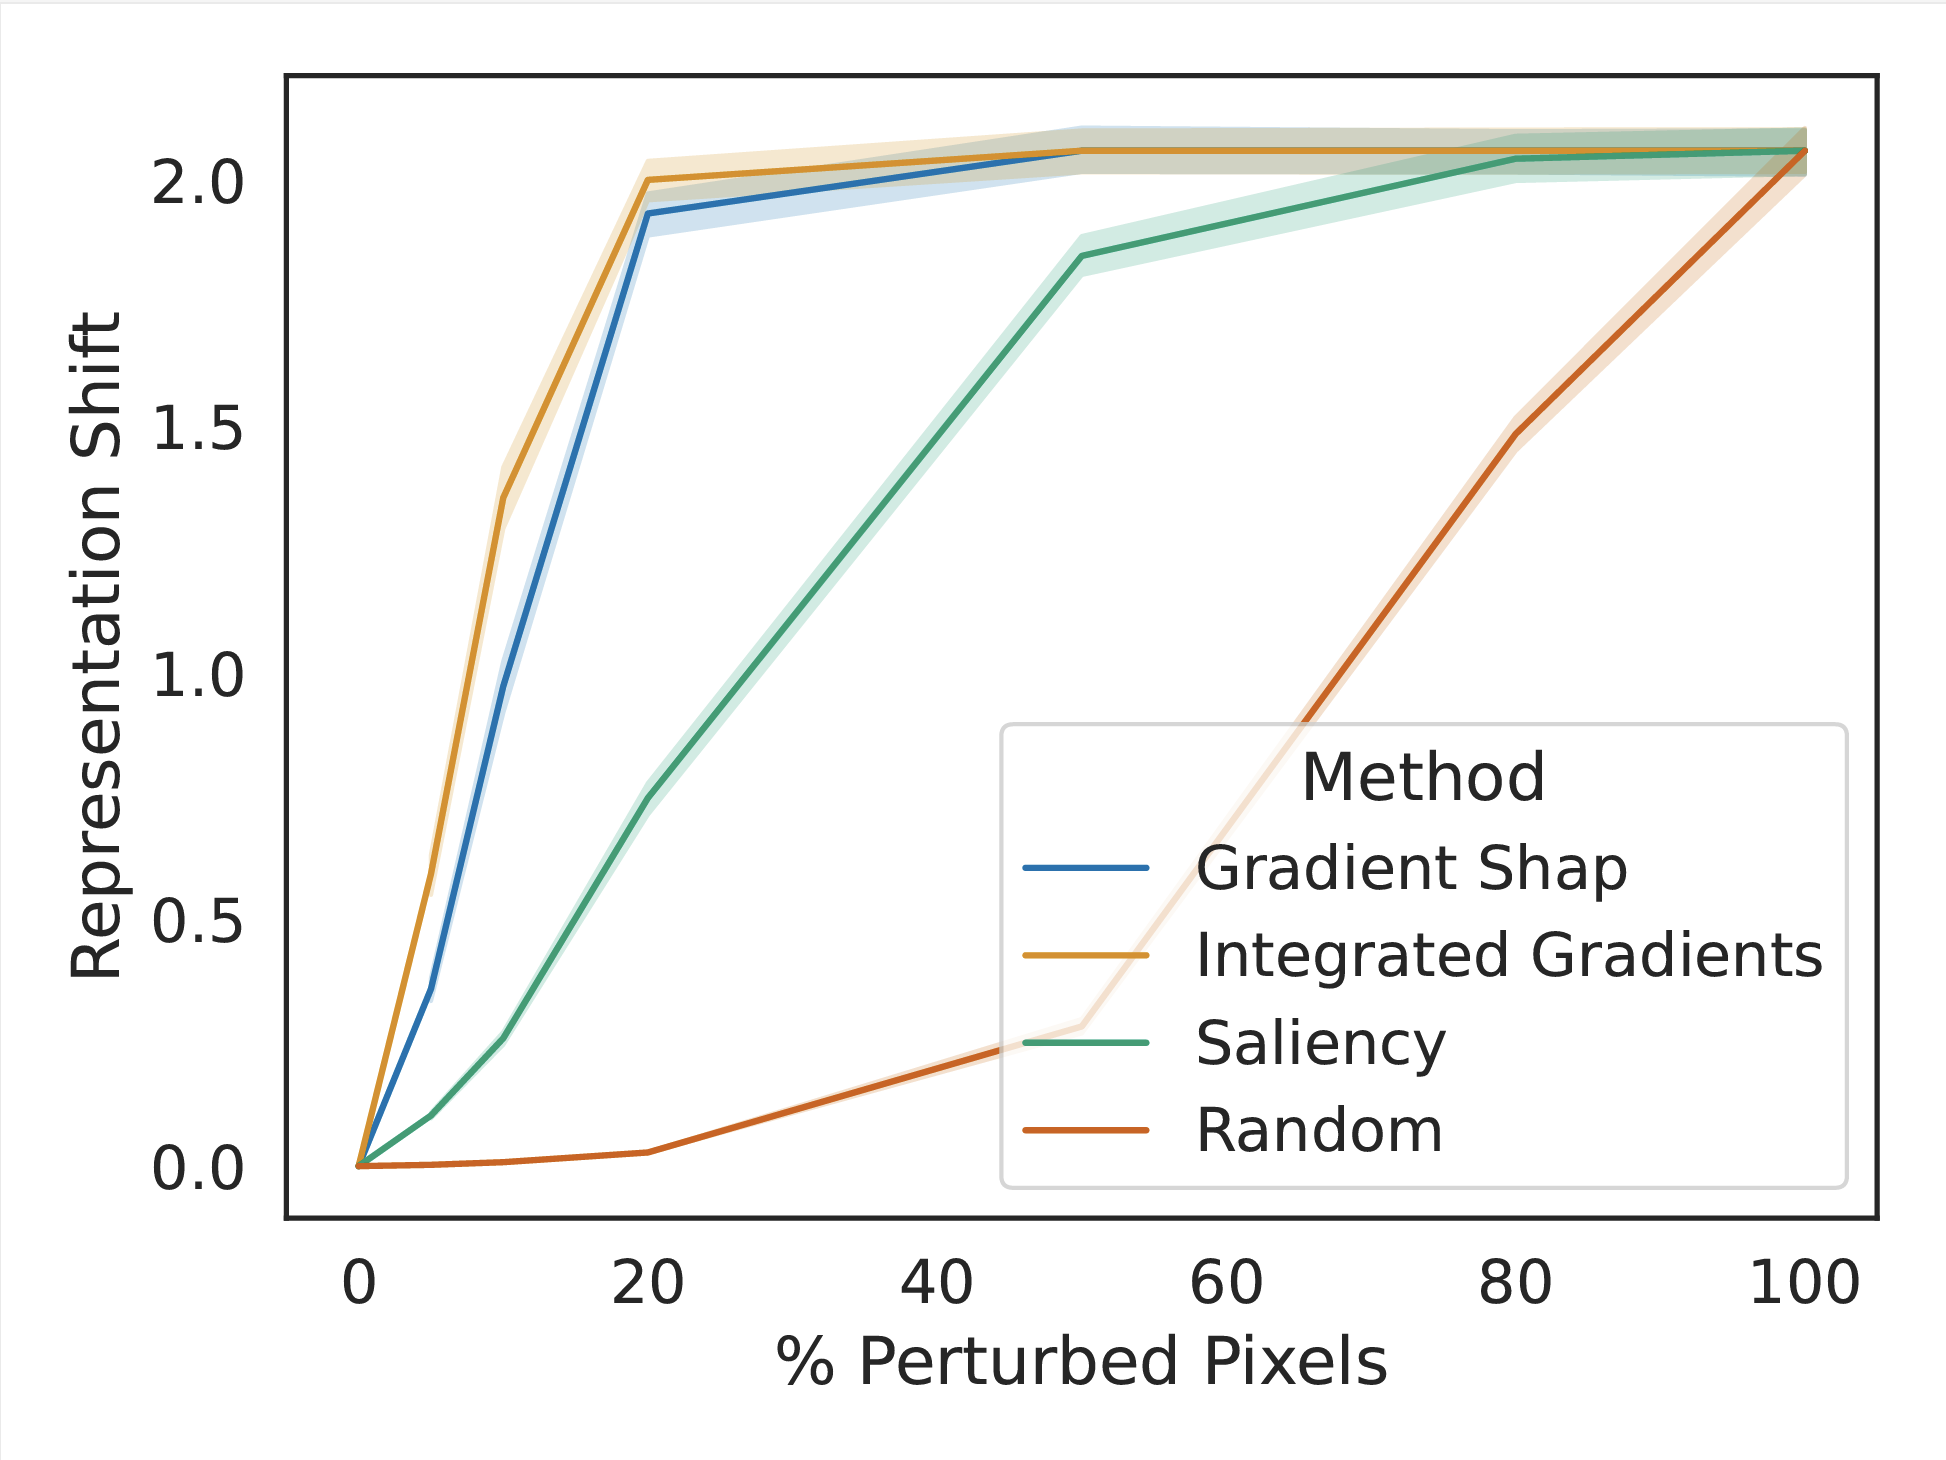
\includegraphics[width=\textwidth]{images/feature_consistency_mnist.png}
         \caption{MNIST}
         \label{fig:feature_consistency_mnist}
     \end{subfigure}
     \hfill
     \begin{subfigure}[b]{0.3\textwidth}
         \centering
         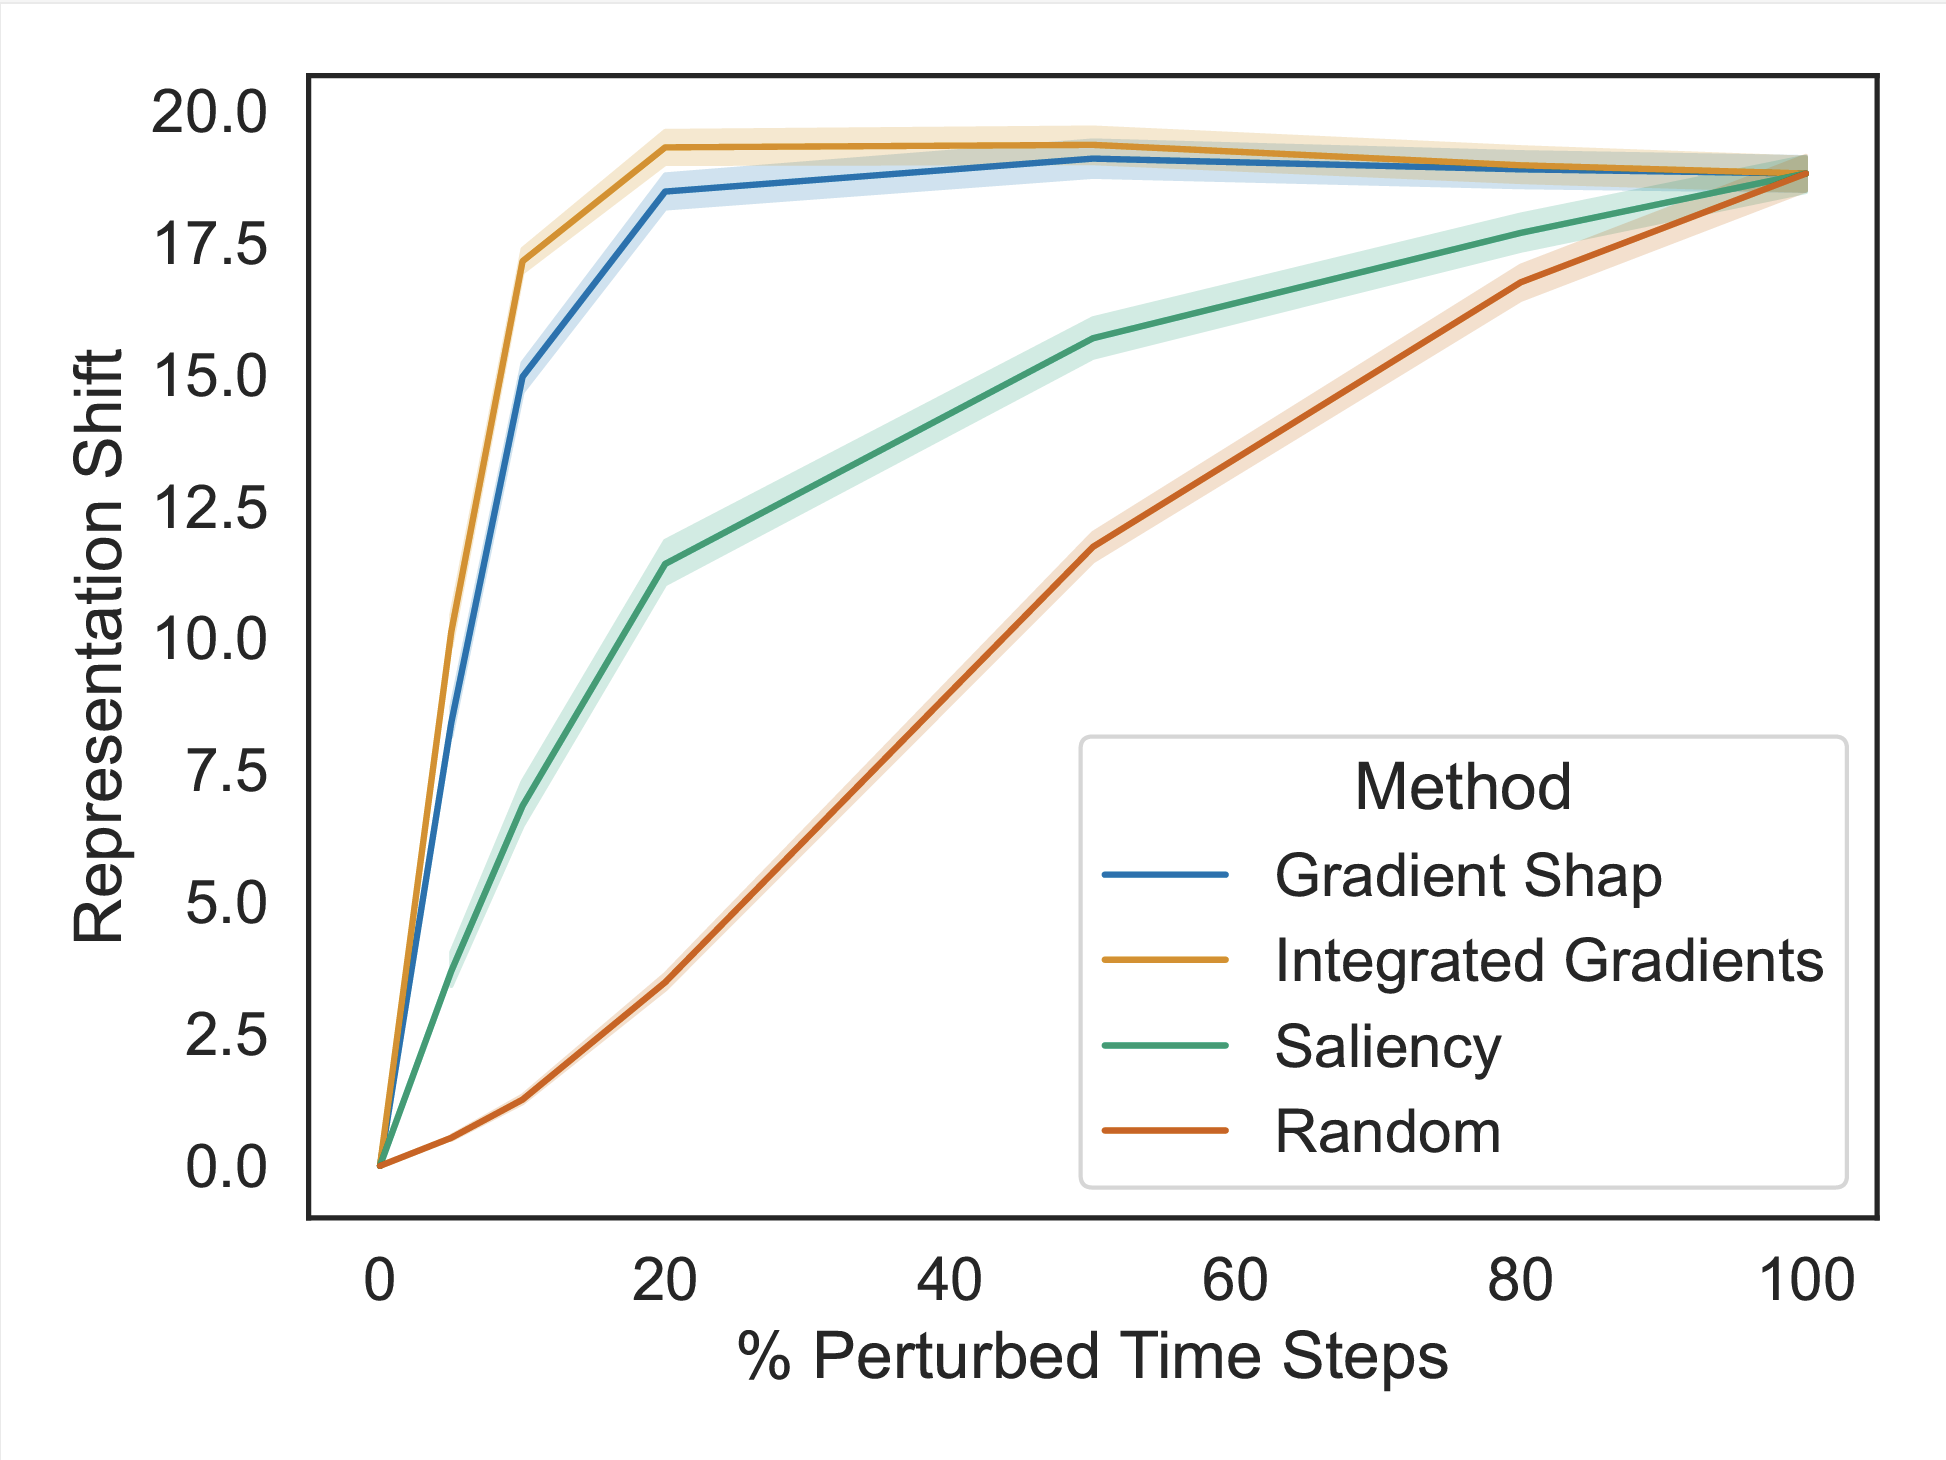
\includegraphics[width=\textwidth]{images/feature_consistency_ecg5000.png}
         \caption{ECG5000}
         \label{fig:feature_consistency_ecg}
     \end{subfigure}
     \hfill
     \begin{subfigure}[b]{0.3\textwidth}
         \centering
         \includegraphics[width=\textwidth]{images/feature_consistency_cifar.png}
         \caption{CIFAR-10}
         \label{fig:feature_consistency_cifar}
     \end{subfigure}
        \caption{Consistency check for label-free feature importance.}
        \label{fig:feature_consistency.png}
\end{figure}



\subsubsection{Example Consistency Checks}
To check whether \textbf{\hyperref[claim2]{claim 2}} holds or not, the authors conducted experiments on three different datasets. The setup for these checks is to sample 1000 training examples and compute the importance score of each in predicting the latent representation of the test images. For computing the score, adaptations to the label-free setting of several methods (both loss and representation based) were used: Influence Functions \cite{cook1980ch}\cite{koh}, TracIn \cite{pruthi}, SimplEx \cite{crabbe}, DKNN \cite{papernot}. In order to check the effectiveness of the methods they selected the $M$ most important training examples and computed the similarity rates between them. They did the same for the $M$ least important examples and expected the similarity between the least important samples to be lower than between the most important ones. Figure \ref{fig:example-importance} shows the results we obtained after reproducing the original experiments on MNIST, ECG5000 and CIFAR-10 datasets. The plots display the distribution of similarity rates for different values for $M$ and example importance methods. For MNIST and ECG5000 our results match the ones from the paper, but for CIFAR-10, even though the trend is similar, the scale of the similarity rate differs, as for us it peaks at 0.5, while in the original paper, the highest value is around 0.17. All in all, our results validate \textbf{\hyperref[claim2]{claim 2}} which states that label-free importance scores allow us to determine the training examples that explain the test ones best.
\begin{figure}
     \centering
     \begin{subfigure}[b]{0.3\textwidth}
         \centering
         \includegraphics[width=\textwidth]{images/example_consistency_mnist.png}
         \caption{MNIST}
         \label{fig:mnist1}
     \end{subfigure}
     \hfill
     \begin{subfigure}[b]{0.3\textwidth}
         \centering
         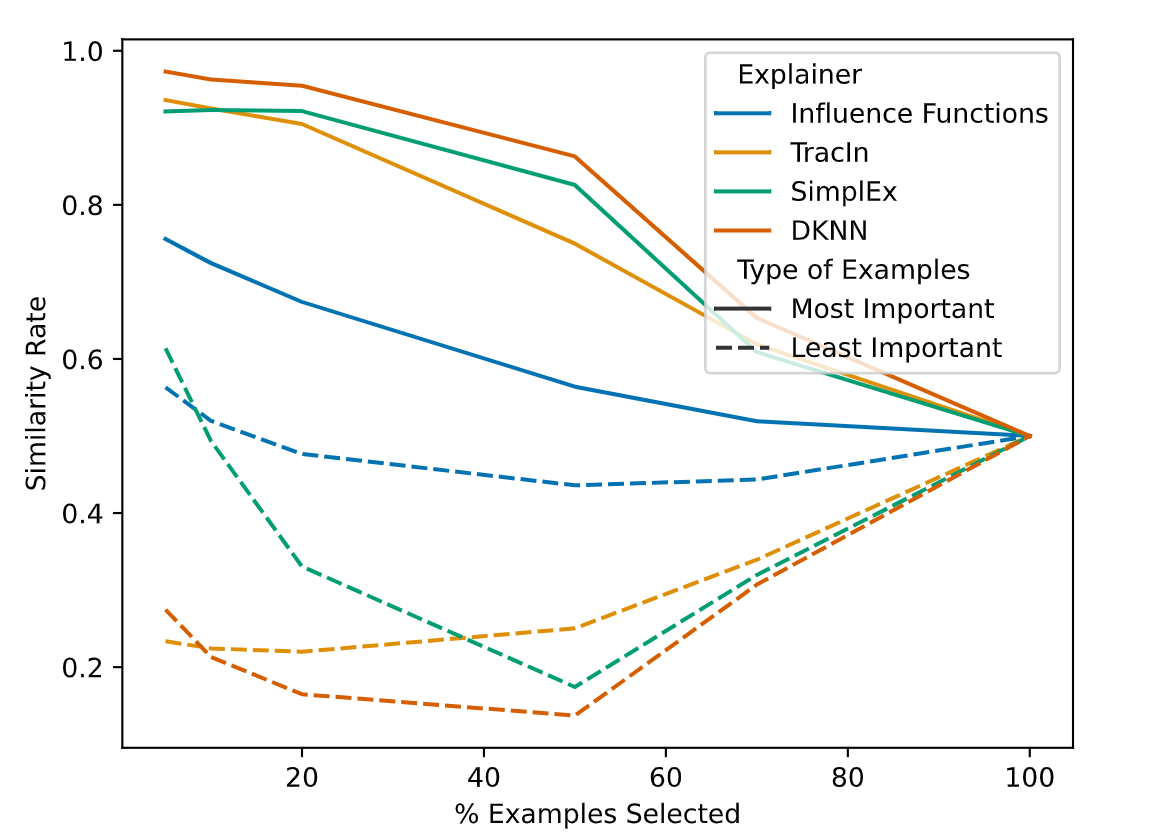
\includegraphics[width=\textwidth]{images/example_consistency_ecg.png}
         \caption{ECG5000}
         \label{fig:ecg1}
     \end{subfigure}
     \hfill
     \begin{subfigure}[b]{0.3\textwidth}
         \centering
         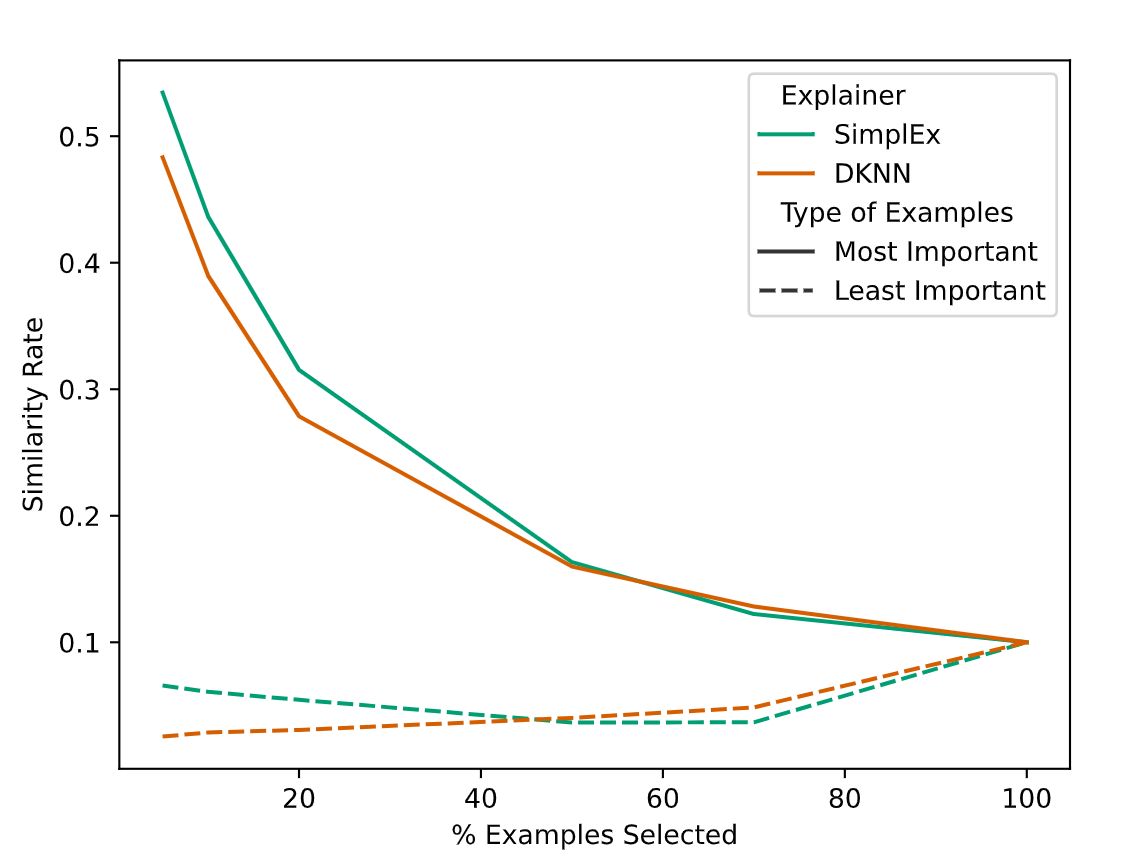
\includegraphics[width=\textwidth]{images/example_consistency_cifar10.png}
         \caption{CIFAR-10}
         \label{fig:cifar}
     \end{subfigure}
        \caption{Consistency check for label-free example importance.}
        \label{fig:example-importance}
\end{figure}

\subsubsection{Comparing the Representations Learned with Different Pretext Tasks}
%Mara

To support \textbf{\hyperref[claim1]{claim 1}} and \textbf{\hyperref[claim2]{claim 2}}, the authors compared different pretext tasks, such as denoising, reconstruction, and inpainting, qualitatively and quantitatively. Through this analysis, they support \textbf{\hyperref[claim3]{claim 3}}. We reproduce the experiments in the same way, by using the MNIST dataset and averaging the Pearson correlation coefficients of five runs of different autoencoders, as stated in the original paper in Appendix C.2. For the \textbf{quantitative analysis}, we focus on interpreting and comparing the Pearson correlation obtained for feature and example importance shown in Table \ref{table:pc_saliency_reproduced} and Table \ref{table:pc_example_reproduced}, respectively, with the results from the original paper. In our case, the Pearson correlation coefficients for saliency maps range from .32 to .43 corresponding to the moderate positive correlations also obtained in the original paper. Furthermore, we have Pearson correlation coefficients for example importance ranging from .05 to .13 corresponding to the weak correlations obtained in the original paper.


\begin{table}[H]
\footnotesize
    \begin{subtable}[h]{0.5\linewidth}
        \centering
        \begin{tabular}{llll}
        \hline
                        Pear. & Rec. & Den. & Inp.   \\
        \hline
         
         Den.     & $0.38 \pm 0.02$  & &     \\
         Inp.   & $0.33 \pm 0.05$  & $0.32 \pm 0.02$ &    \\
         Clas.   & $0.43 \pm 0.02$  & $0.4 \pm 0.01$  & $0.35 \pm 0.04$     \\
        \hline
        \end{tabular}
    \caption{Pearson correlation for saliency maps (avg +/- std).}
    \label{table:pc_saliency_reproduced}
    \end{subtable}
    \begin{subtable}[h]{0.5\linewidth}
        \centering

        \begin{tabular}{llll}
        \hline
                        Pear. & Rec. & Den. & Inp.  \\
        \hline
         
         Den.    & $0.08 \pm 0.04$  &  &    \\
         Inp.   & $0.13 \pm 0.05$  & $0.09 \pm 0.01$ &   \\
         Clas.   & $0.07 \pm 0.02$  & $0.05 \pm 0.02$ & $0.08 \pm 0.02$   \\
        \hline
            \end{tabular}
        
    \caption{Pearson correlation for example imp. (avg +/- std).}
    \label{table:pc_example_reproduced}
    \end{subtable}
    \caption{Pretext experiment results.}
\end{table}

In terms of the \textbf{qualitative analysis}, we plot the most important examples and saliency maps for different encoders to support \textbf{\hyperref[claim2]{claim 2}} and \textbf{\hyperref[claim3]{claim 3}}. Visually, one can interpret the saliency maps as being different from one pretext task to another. Moreover, the top examples produced by different pretext tasks are hardly similar. Both conclusions reinforce the previous results from the quantitative analysis and compare positively to the results from the paper. Examples of these visualizations are shown in Appendix \ref{appendix:pretext_visualisations}. In conclusion, the representations of different pretext tasks are not interchangeable.



\subsubsection{Challenging Assumptions with Disentangled VAEs} 
 To investigate the paper's \textbf{\hyperref[claim4]{claim 4}}, we trained two disentangled VAEs, $\beta$-VAE and TC-VAE on MNIST and dSprites datasets.
 For the \textbf{qualitative Analysis}, we have validated the three paper's conclusions. Saliency maps of four test images are shown in Figure \ref{fig:saliencyVAE}. Firstly, the latent unit can be sensitive and insensitive to similar images (Latent Unit 2 of the MNIST VAE is sensitive to image 1 but not to Image 2). Secondly, the focus of a latent unit can be completely different between similar images (Latent unit 5 of dSprites VAE in Image 1 focuses on the interior of the rectangle, and in Image 2 it focuses on the border of the rectangle). Lastly, some latent units focus on the same part of the image  (Image 3 of MNIST). In terms of the \textbf{quantitative Analysis}, box plots observed in Figure \ref{fig:pearsonVAE} have some differences from the ones in the paper. That could be normal given how unstable and hard to seed VAEs are. Regarding the dSprites dataset, the plot shows a moderate increase in the Pearson correlation coefficients with $\beta$. Concerning the MNIST dataset, we observed a slight decrease in Pearson correlation with $\beta$. That leads us to the conclusion that increasing $\beta$ does not suggest that latent units are paying attention to a specific part of the image, which is the same conclusion as in the paper.

%  \begin{figure}[H]
%     %\centering
%     \includegraphics[width=13cm]{images/Saliency-VAE.png}
%     \caption{ Saliency map for each unit of the disentangled VAEs. }
%     \label{fig:saliencyVAE.png}
%     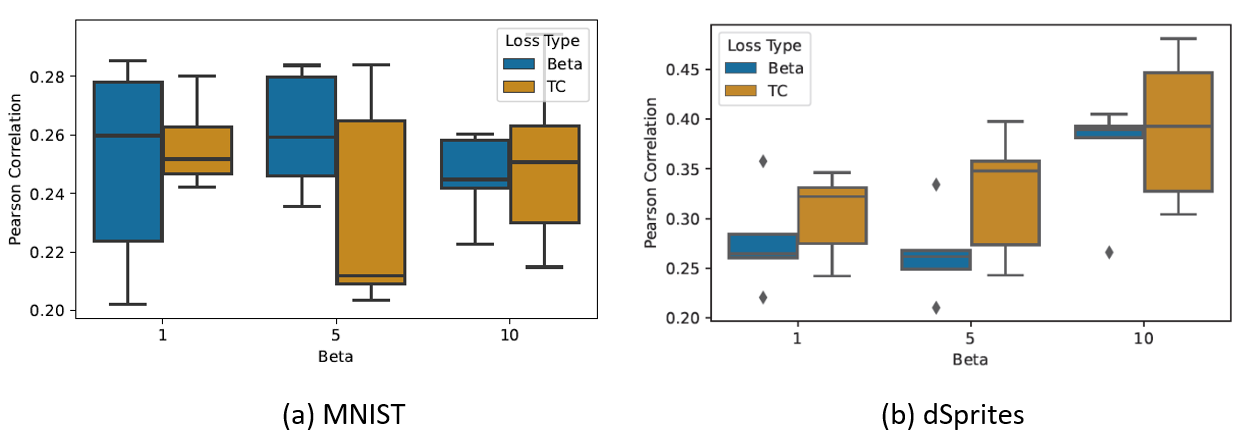
\includegraphics[width=13cm]{images/PearsonCorrelationBetas.png}
%     \caption{ Pearson correlation between saliency maps for different values of $\beta$. }
%     \label{fig:pearsonVAE.png}
% \end{figure}

\begin{figure}[H]
     \begin{subfigure}[b]{0.365\textwidth}
         \centering
         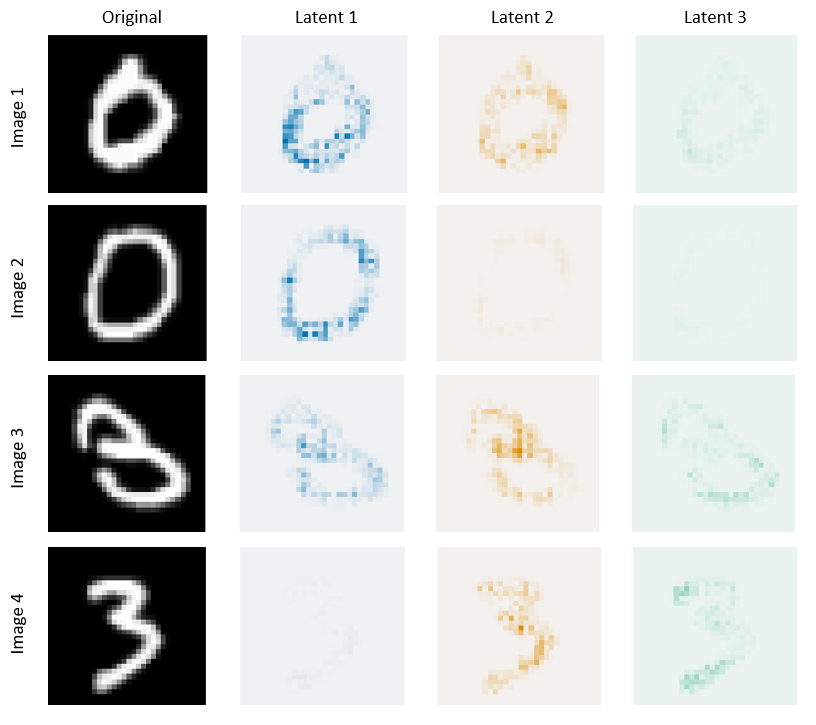
\includegraphics[width=\textwidth]{images/saliency_Mnist.png}
         \caption{MNIST}
         \label{fig:saliencyMNIST}
     \end{subfigure}
     \hfill
     \begin{subfigure}[b]{0.635\textwidth}
         \centering
         \includegraphics[width=\textwidth]{images/sasliency_dsprites.png}
         \caption{dSprites}
         \label{fig:dsprites}
     \end{subfigure}
        \caption{Saliency maps for each unit of the disentangled VAEs.}
        \label{fig:saliencyVAE}
\end{figure}

\begin{figure}[H]
     \begin{subfigure}[b]{0.45\textwidth}
         \centering
         \includegraphics[width=\textwidth]{images/PearsonMnist.png}
         \caption{MNIST}
         \label{fig:CIFARpearsonVAE}
     \end{subfigure}
     \hfill
     \begin{subfigure}[b]{0.45\textwidth}
         \centering
         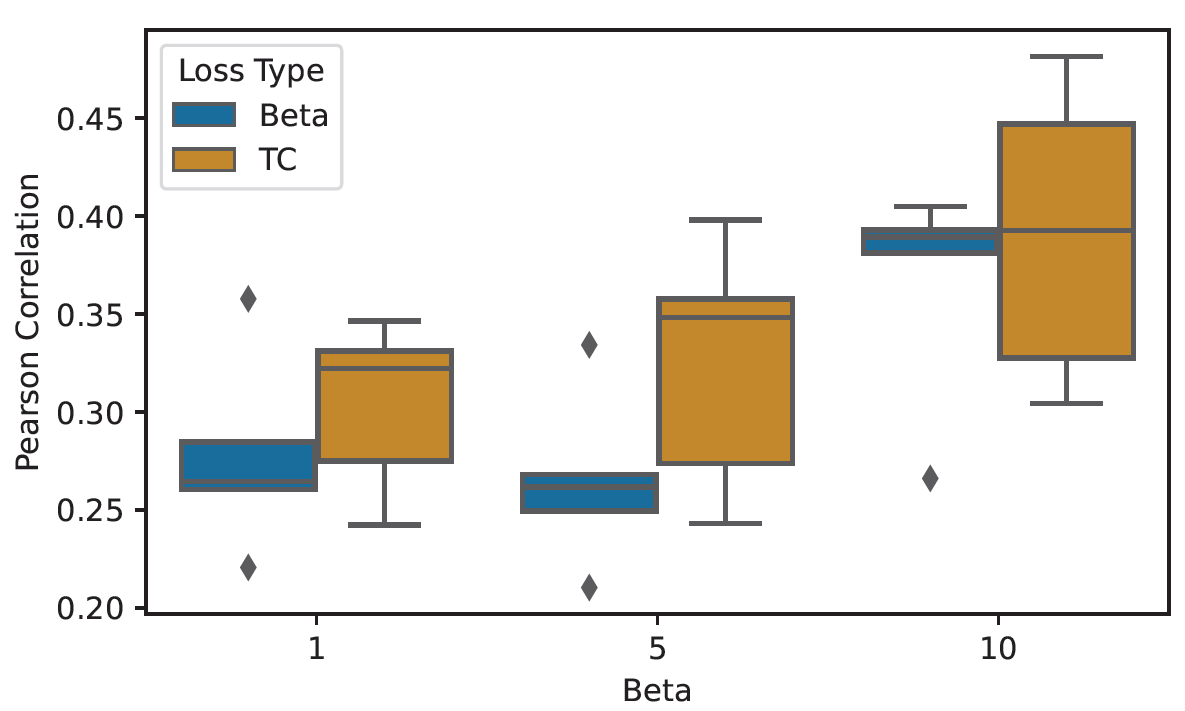
\includegraphics[width=\textwidth]{images/PearsonDsprites.png}
         \caption{dSprites}
         \label{fig:pearson}
     \end{subfigure}
        \caption{Pearson correlation between saliency maps for different values of $\beta$.}
        \label{fig:pearsonVAE}
\end{figure}

\subsection{Results beyond original paper}

% Often papers don't include enough information to fully specify their experiments, so some additional experimentation may be necessary. For example, it might be the case that batch size was not specified, and so different batch sizes need to be evaluated to reproduce the original results. Include the results of any additional experiments here. Note: this won't be necessary for all reproductions.

\subsubsection{Fashion MNIST}
% Ana

In order to test the generalizability of the methods, we run the feature and example importance experiments on a different dataset, Fashion MNIST. We also compared both quantitatively and qualitatively the representations learned for several pretext tasks and questioned how different the representations are from each other by computing their Pearson correlation coefficient and plotting the most important samples and the saliency maps. The feature importance graph can be seen in Figure \ref{fig:fashion_mnist_f_imp} and it shows that the representation shift increases abruptly when we perturb the most important pixels, following the same trend as for the other datasets. The example importance graphs along with the correlation coefficients and plots can be seen in detail in Appendix \ref{appendix:pretext_visualisations_fmnist}. The results for Fashion MNIST reinforce the idea that encoders trained on different pretext tasks pay attention to distinct features in the image and that the learned representations are not interchangeable.

\begin{figure}
     \centering
     \begin{subfigure}[b]{0.3\textwidth}
         \centering
         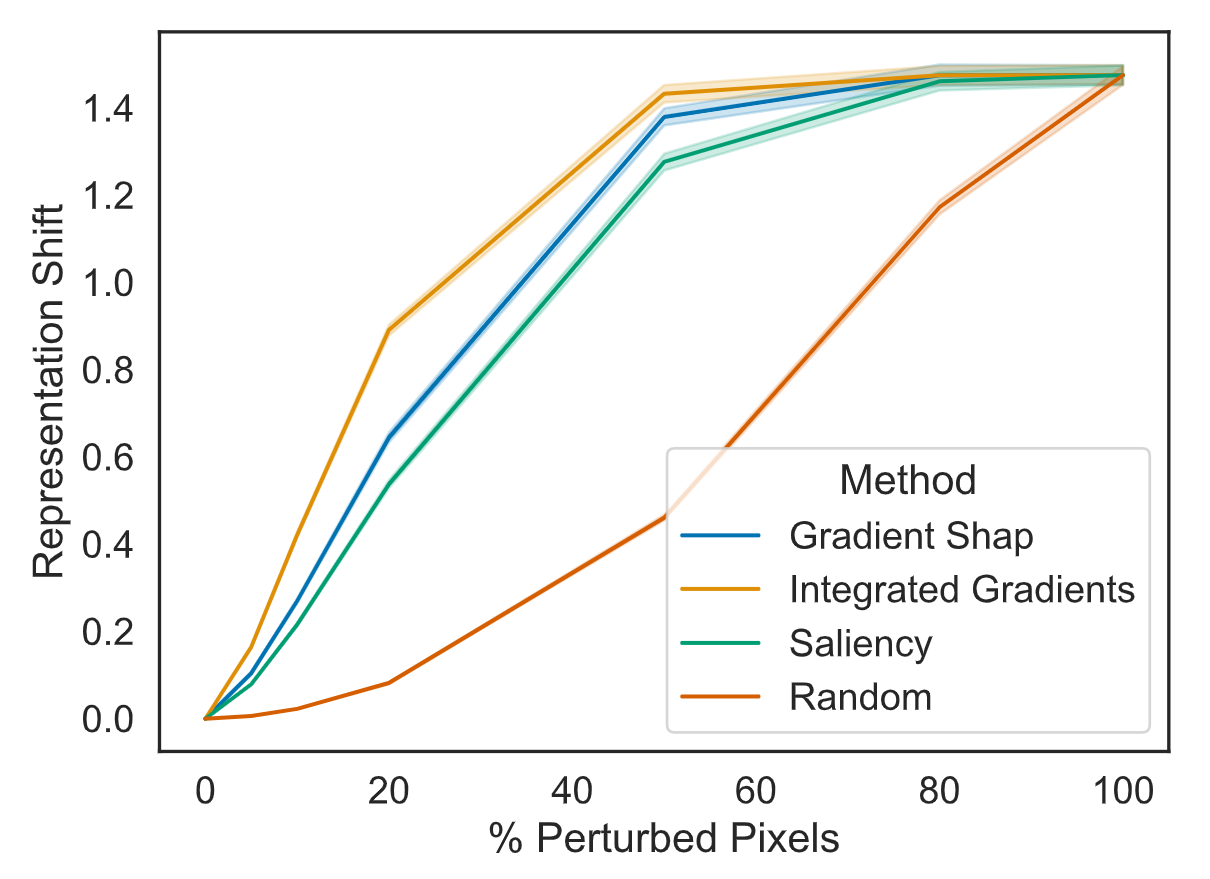
\includegraphics[width=\textwidth]{images/feature_consistency_fmnist.png}
         \caption{Fashion MNIST.}
         \label{fig:fashion_mnist_f_imp}
     \end{subfigure}
     \hfill
     \begin{subfigure}[b]{0.3\textwidth}
         \centering
         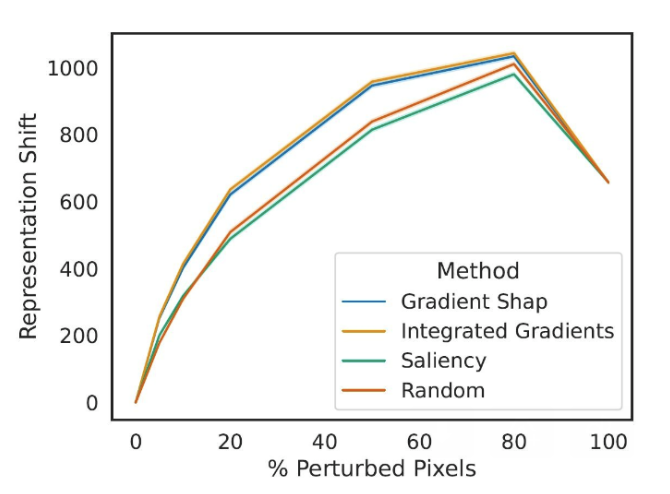
\includegraphics[width=\textwidth]{images/black pixels.png}
         \caption{CIFAR-10: black pixel masks.}
         \label{black_pixels}
     \end{subfigure}
     \hfill
     \begin{subfigure}[b]{0.3\textwidth}
         \centering
         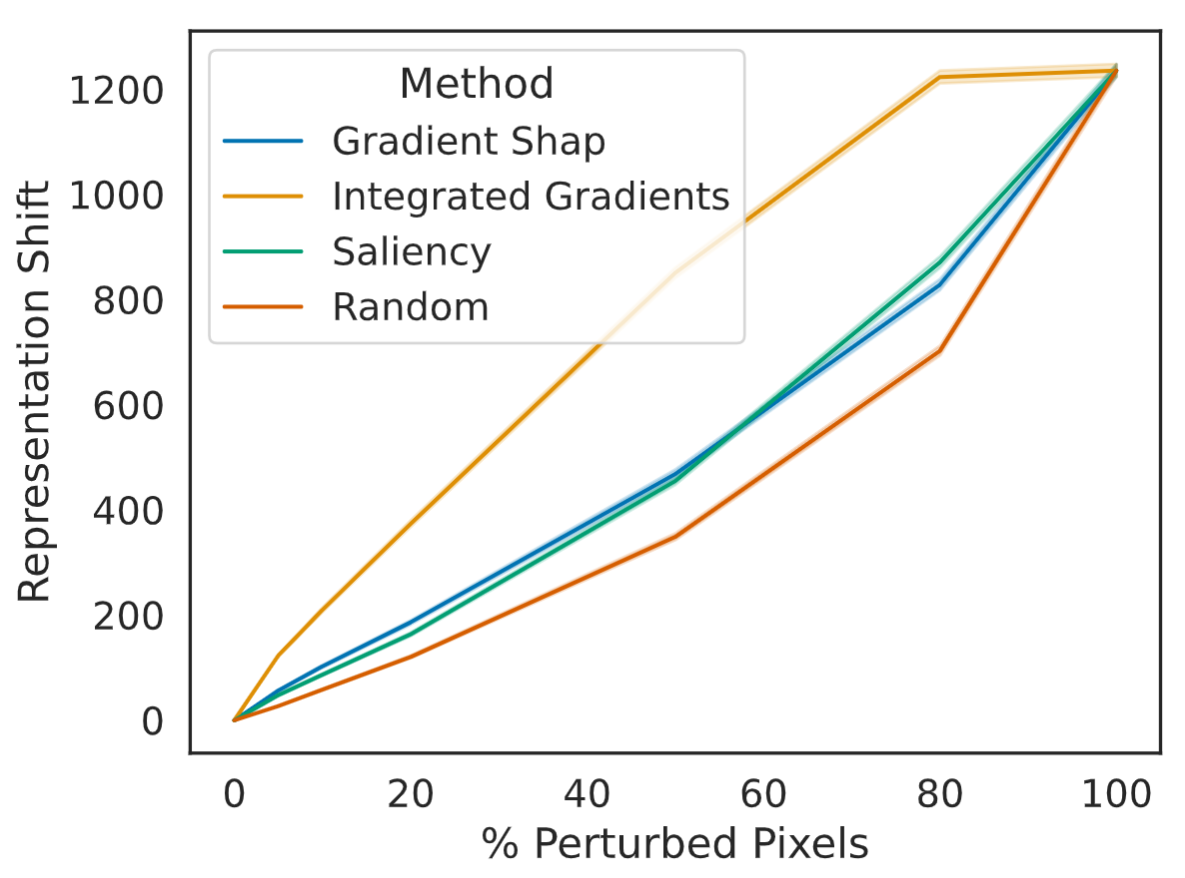
\includegraphics[width=\textwidth]{images/feature_consistency_dense.png}
         \caption{CIFAR-10: DenseNet encoder.}
         \label{fig:densenet_f_imp}
     \end{subfigure}
        \caption{Consistency check for label-free feature importance on additional experiments.}
        \label{fig:feat-importance-fashion-dense}
\end{figure}

\subsubsection{Additional experiments for CIFAR-10 dataset} 



In section \ref{section41} evaluating \textbf{\hyperref[claim1]{claim 1}}, we mentioned that we found inconsistencies between the original and our results for the CIFAR-10 dataset. We decided to investigate further this experiment. As a first step, we plotted the masked images to confirm that the quantitative analysis is correct. These results can be found in Figure \ref{fig:blurred_horse}. According to the results, the Integrated Gradients method worked best because most of the pixels covered are on the object, while for the other methods, a lot of pixels identified as salient are in the background. This observation matches the quantitative results presented in section \ref{section41}. In addition, we experimented with the \begin{wrapfigure}{}{0.5\textwidth}
    \centering
    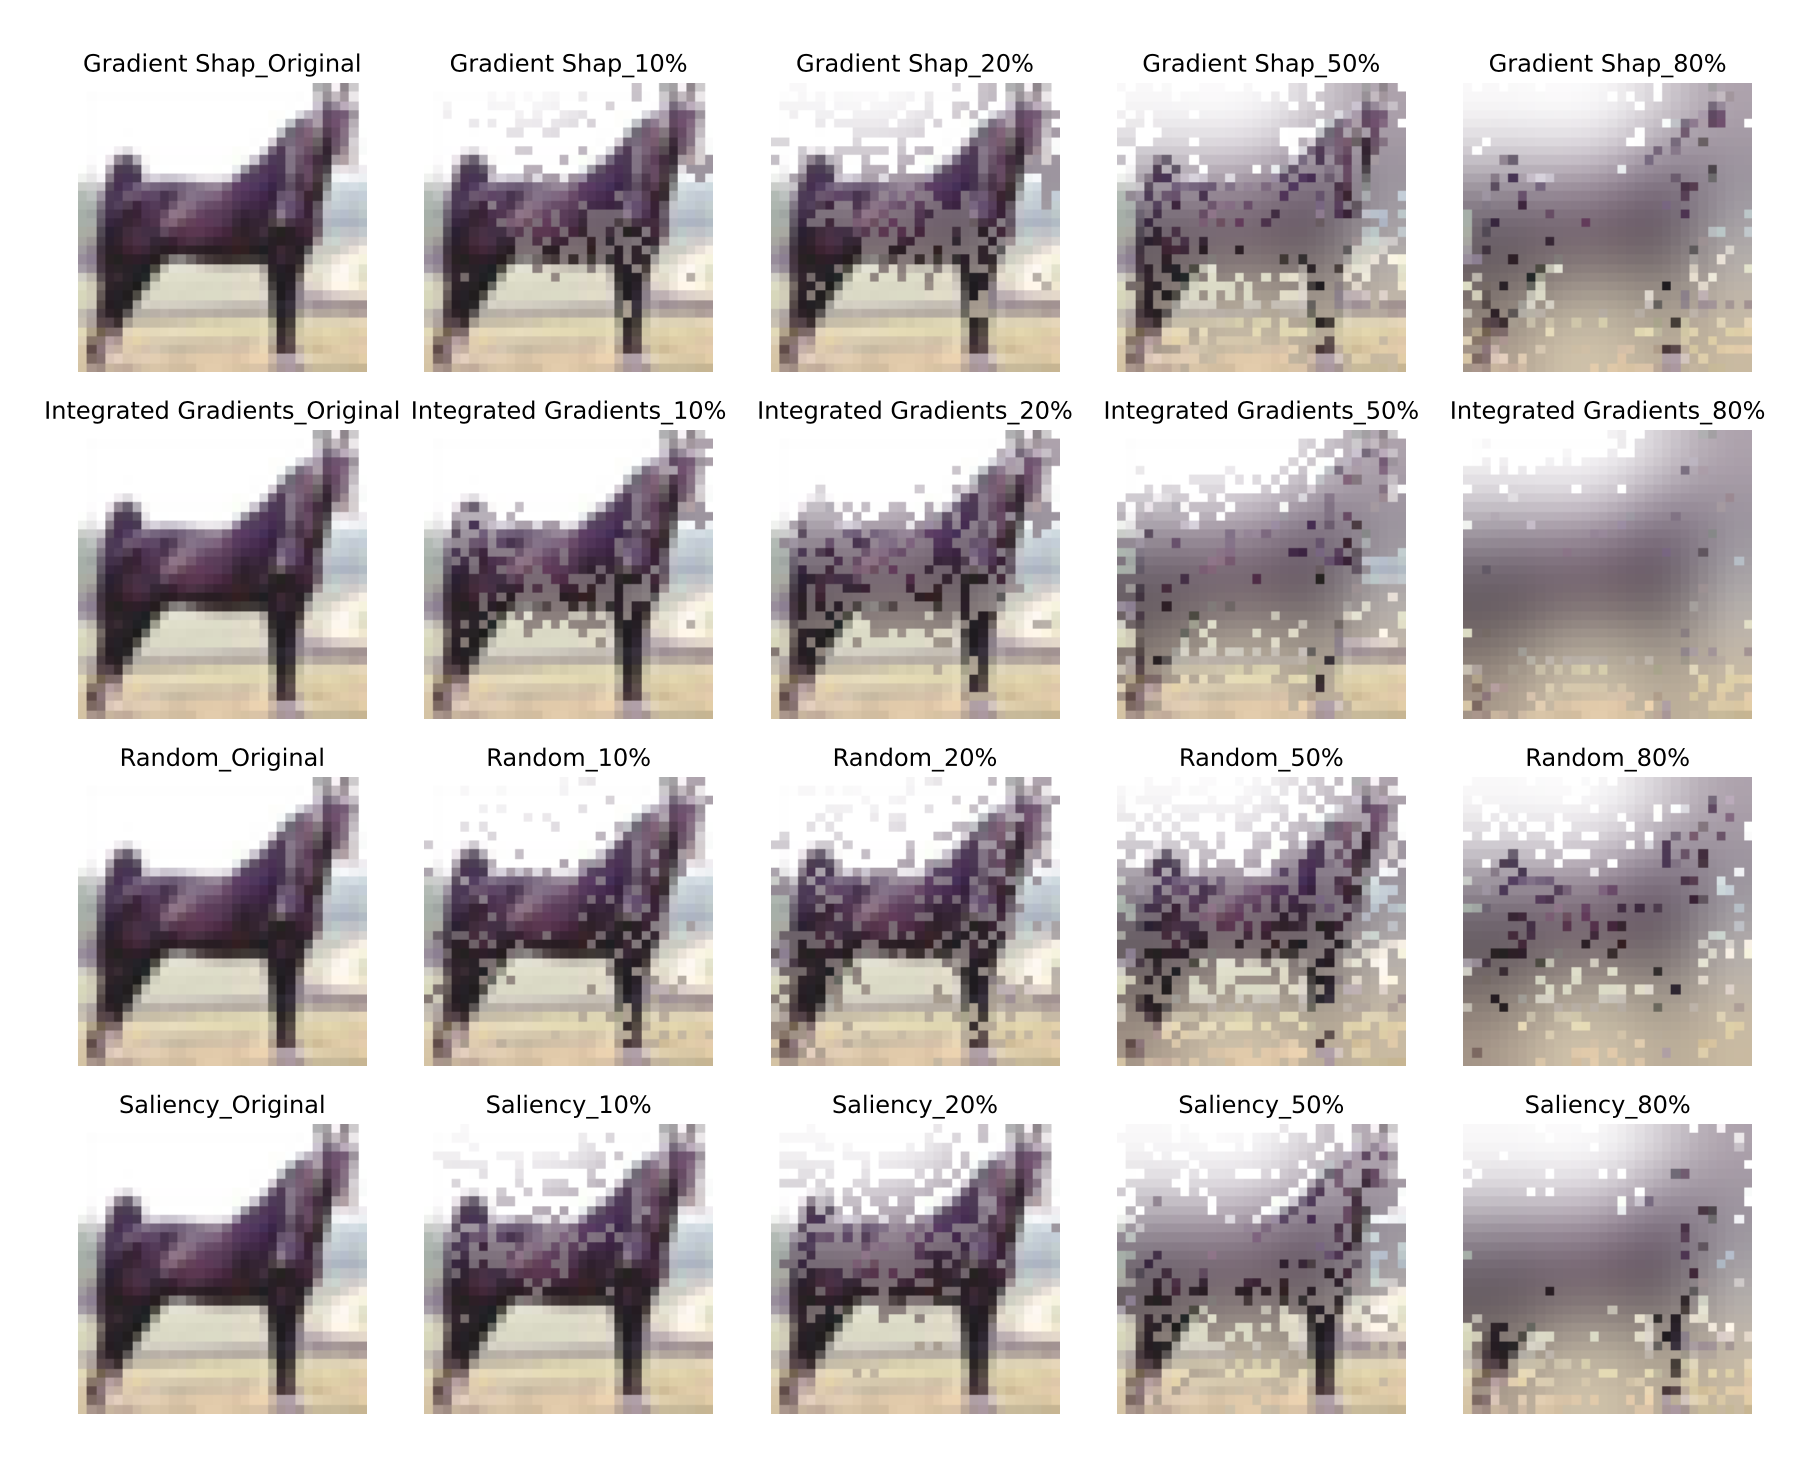
\includegraphics[width=0.47\textwidth]{images/blurred horse.png}
    \caption{Image from CIFAR-10 with blur mask.}
    \label{fig:blurred_horse}
\end{wrapfigure} original pixel-flipping approach proposed by (Montavon et al., 2018)\cite{Montavon} to which the authors referred. This masking method, instead of blurring the most important pixels uses black pixels as a baseline. In Figure \ref{black_pixels} we present the results of this experiment. As we can see Integrated Gradients and Gradient Shap methods performed better in this setup, however the relative difference from the Random baseline method is smaller than previously. We have also decided to plot the masked images which again matched quantitative metrics. Those results are presented in Figure \ref{fig:black_horse} available in the appendix.


% \begin{figure}[H]
%     \centering
%     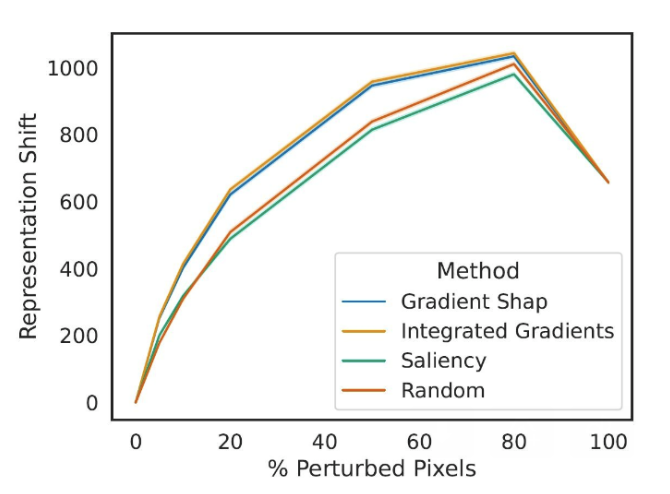
\includegraphics[width=7cm]{images/black pixels.png}
%     \caption{Consistency check for label‐free feature importance on CIFAR-10 with black pixels masks.}
%     \label{fig:black pixels}
% \end{figure}


\subsubsection{Explainability analysis with different attribution methods}
% Mara

% We asked the authors about the choice, and the reason for using Gradient Shap is because it is faster than Integrated Gradients

The authors concluded after the feature consistency checks that the \textit{label-free Integrated Gradients outperforms other methods for each model} tested. However, for their pretext and VAE tests, they used label-free Gradient Shap to produce the saliency maps. In this experiment, we want to observe the generalizability of the label-free feature importance in the context of self-supervised learning and disentangled VAEs. We experiment with label-free Integrated Gradients by using it as an attribution method for label-free feature importance. The experimental settings remain the same as described for the pretext and VAE experiment, respectively. The quantitative and qualitative results for each attribution method are shown in Appendix \ref{appendix:explainability_attr_methods}. We obtain the same conclusion about the medium Pearson correlation for the feature importance and the low correlation for the example importance as in the original paper. For the VAE experiment, the Pearson correlation coefficients have higher values compared to the ones obtained using Gradient Shap in the original paper. However, we observe that as \( \beta \) grows, latent units are not paying attention to distinct parts of the image because the Pearson correlation does not decrease at the same time with \(\beta\). Therefore, we could conclude both the pretext and VAE experiments similarly as in the original experiments, using label-free Integrated Gradients instead of label-free Gradient Shap, enhancing \textbf{\hyperref[claim1]{claim 1}}. This also proves the \textit{generalizability} of the label-free feature importance, which is an easy-to-adapt method to practical examples and existing supervised explainability methods.

\subsubsection{Evaluating CIFAR-10 experiments using DenseNet}
 % Andreas
 
 To validate the integrity of \textbf{\hyperref[claim1]{claim 1}} and \textbf{\hyperref[claim2]{claim 2}} further in terms of the model used, we decided to change the encoder of the SimCLR network from a ResNet18 (or 34) to a DenseNet121. By running the same experiments we obtained identical results as can be seen in Figure \ref{fig:densenet_f_imp}. The results can be found in the appendix (Figure \ref{fig:cifar_densenet}). The trends are the same as the ones using the ResNet encoder, designating that the conclusion does not depend on the encoder.
 

% We found that the explainability methods generalize to new datasets, as the results for Fashion MNIST followed the same trends for all the experiments as the other datasets did.

\section{Discussion}

% Give your judgement on if your experimental results support the claims of the paper. Discuss the strengths and weaknesses of your approach - perhaps you didn't have time to run all the experiments, or perhaps you did additional experiments that further strengthened the claims in the paper.

In this study, we carried out multiple experiments to replicate the key findings from the original research. Our reproducibility results lend credence to the original claims, as we were able to largely replicate the original findings. We validated the four claims of the authors, except for some minor discrepancies on CIFAR-10. Regarding these inconsistencies, we decided to contact the authors, and they provided us with the pre-trained model they used to perform experiments in the original paper. With the use of this model, we were able to obtain the same results as the authors, however, we couldn't reproduce them by training the model on our own. Additionally, we asked the authors why they choose to blur pixels instead of changing them to black. They justified it by pointing out that for the CIFAR-10 dataset, some black pixels may be salient, which will result in zero attribution. We confirmed that by looking at the results, however the parameters for Gaussian Blur were handcrafted and might not generalize well to different datasets. Aiming to prove the robustness of the proposed frameworks for a label-free feature and example importance we decided to test them in different settings. Firstly, we used a different dataset, the Fashion MNIST dataset, and we were able to prove that the conclusions still hold. Secondly, by swapping the encoder of SimCLR from ResNet to DenseNet we proved that the results are not dependent on the encoder. Furthermore, we experimented with a different attribution in the practical example of pretext tasks in self-supervised learning and VAE challenge, namely label-free Integrated Gradients instead of Gradient Shap, to support the generability of the label-free feature importance.

% \subsection{What was easy}

% Give your judgement of what was easy to reproduce. Perhaps the author's code is clearly written and easy to run, so it was easy to verify the majority of original claims. Or, the explanation in the paper was really easy to follow and put into code. 

% Be careful not to give sweeping generalizations. Something that is easy for you might be difficult to others. Put what was easy in context and explain why it was easy (e.g. code had extensive API documentation and a lot of examples that matched experiments in papers). 

% \subsection{What was difficult}

% List part of the reproduction study that took more time than you anticipated or you felt were difficult. 

% Be careful to put your discussion in context. For example, don't say "the maths was difficult to follow", say "the math requires advanced knowledge of calculus to follow".



\subsection{Reflection: What was easy, and what was difficult?}
The original paper had all the newly introduced methods and experiments clearly stated and further explained in the appendix with mathematical proofs, detailed architectures of the models, values for hyperparameters and qualitative results. On top of this, having access to the original code implementation made it easy and straightforward to run all the experiments. The datasets were also publicly available. Even though the code was available and most of the reproducibility experiments were done without any modifications, the comments in the code were too sparse; therefore, understanding and extending the code demanded more time than expected. Moreover, the ECG5000 example importance experiments required more than the maximum time that we could use the GPU continuously. Thus, we modularized the code to save intermediate results which we merged together in the end.
\subsection{Communication with original authors}

% Document the extent of (or lack of) communication with the original authors. To make sure the reproducibility report is a fair assessment of the original research we recommend getting in touch with the original authors. You can ask authors specific questions, or if you don't have any questions you can send them the full report to get their feedback before it gets published. 
 

We raised questions about some differences in the results, explored explanations for implementation decisions, and then got in touch with the authors for clarification. The authors replied immediately and provided satisfactory answers to most of our questions. However, a few of the answers were not sufficient. For instance, concerning the differences in the results using CIFAR-10 dataset, the authors provided the specific file with the trained parameters that were used for obtaining the results in the original paper. We were able to reproduce the original results using the pretrained model given by the authors. However, we were not able to find what exactly is causing the difference; we believe that they used different hyperparameters than specified in the paper.


